\documentclass[border=10pt]{standalone}

\usepackage{tikz}
\usepackage{tikzsymbols}
\usetikzlibrary{calc,patterns,shapes.geometric}

\def\centerarc[#1](#2)(#3:#4:#5){\draw[#1] ($(#2)+({#5*cos(#3)},{#5*sin(#3)})$) arc (#3:#4:#5);}

\begin{document}
	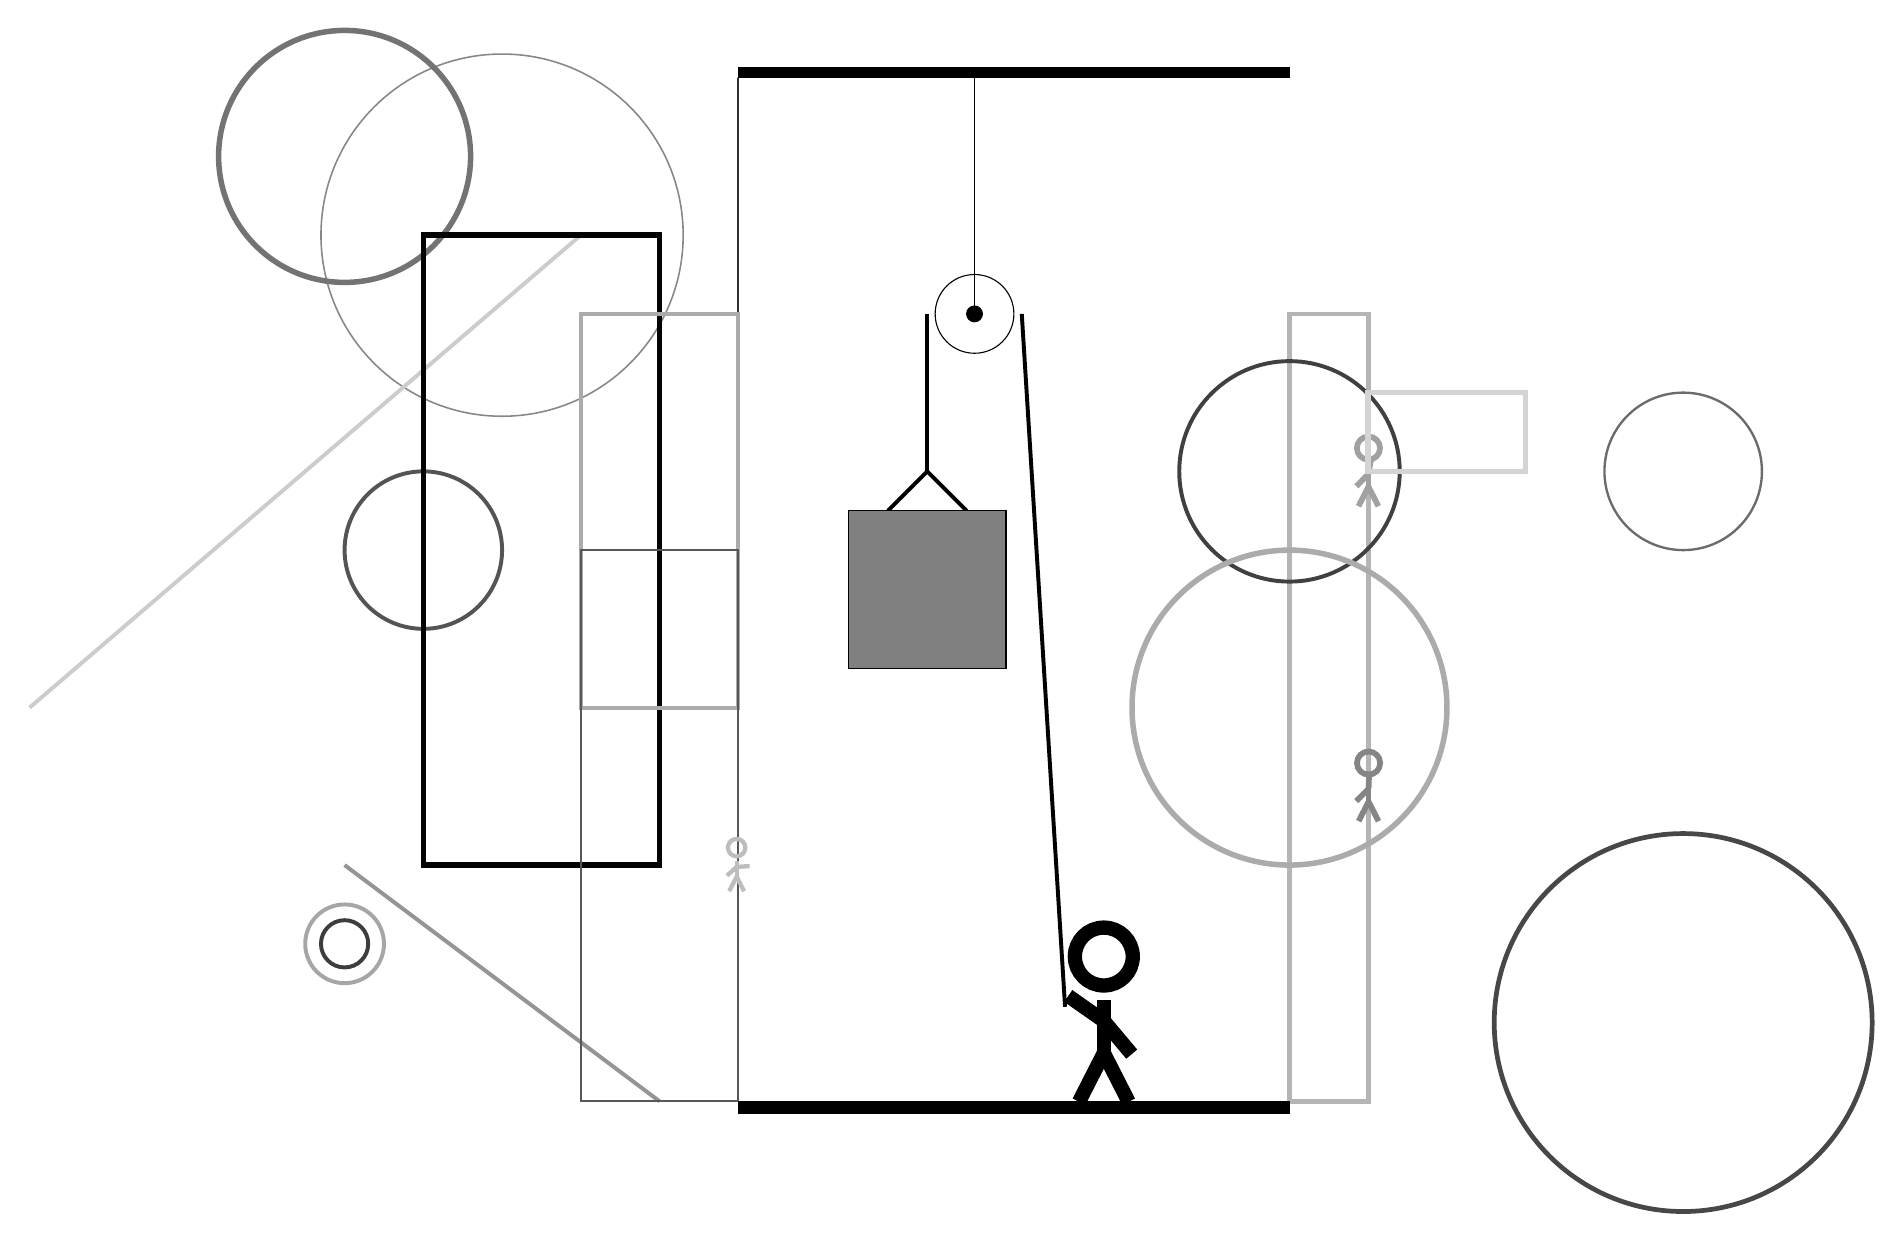
\begin{tikzpicture}
		%%%%% START %%%%%
		
		\draw[fill=black] (-2, 10) rectangle (5, 10.125);
		
		\draw (1, 7) circle (0.5);
		\draw[fill=black] (1, 7) circle (0.1);
		\draw (1, 10) -- (1, 7);
		
		\draw[line width=0.5mm] (-0.1, 4.5) -- (0.4, 5.0) -- (0.9, 4.5);
		\draw[fill=black!50] (-0.6, 4.5) rectangle (1.4, 2.5);
		
		\draw[line width=0.5mm] (0.4, 7) -- (0.4, 5.0);
		\centerarc[line width=0.5mm](1, 7)(0:180:0.6);
		\draw[line width=0.5mm](1.6, 7) -- (2.15, -1.8);
		
		\draw[line width=0.5mm, color=black!86](5, 6) -- (5, -1);
		
		\draw [line width=0.2mm, color=black!47](-5, 8) circle (2.3);
		\draw[line width=0.3mm, color=black!81] (-2, 2) rectangle (-2, 10);
		\draw [line width=0.5mm, color=black!67](-6, 4) circle (1.0);
		
		\draw[line width=0.6mm, color=black!29] (6, -3) rectangle (5, 7);
		\draw [line width=0.6mm, color=black!72](10, -2) circle (2.4);
		
		\draw[line width=0.5mm, color=black!42](-3, -3) -- (-7, 0);
		\draw[line width=0.5mm, color=black!20](-4, 8) -- (-11, 2);
		\node[line width=0.3mm, color=black!37] at (6, 5) {\Strichmaxerl[4][46][80]};
		\draw [line width=0.3mm, color=black!58](10, 5) circle (1.0);
		\draw [line width=0.7mm, color=black!55](-7, 9) circle (1.6);
		
		\draw[line width=0.7mm, color=black!99] (-3, 8) rectangle (-6, 0);
		\draw[line width=0.5mm, color=black!33] (-2, 7) rectangle (-4, 2);
		
		\draw[line width=0.3mm, color=black!66] (-4, -3) rectangle (-2, 4);
		\draw [line width=0.5mm, color=black!75](5, 5) circle (1.4);
		\node[line width=0.3mm, color=black!48] at (6, 1) {\Strichmaxerl[4][45][88]};
		
		\draw [line width=0.5mm, color=black!76](-7, -1) circle (0.3);
		
		\draw [line width=0.7mm, color=black!33](5, 2) circle (2.0);
		\node[line width=0.4mm, color=black!26] at (-2, 0) {\Strichmaxerl[3][42][4]};
		
		\draw [line width=0.5mm, color=black!35](-7, -1) circle (0.5);
		\draw[line width=0.7mm, color=black!17] (6, 6) rectangle (8, 5);
		
		
		\node at (2.6, -1.9) {\Strichmaxerl[10][-35][-50]};
		
		\draw[fill=black] (-2, -3) rectangle (5, -3.15);
		
		%%%%% END %%%%%
	\end{tikzpicture}
\end{document}